\documentclass[numbers=noenddot,12pt,a4paper]{scrartcl}
\usepackage[greek,ngerman]{babel}
\usepackage[T1]{fontenc}
\usepackage[utf8]{inputenc}
\usepackage{fullpage}
\usepackage{libertine}
\usepackage{ziffer}
\usepackage{graphicx}
\usepackage{units}
%\usepackage{wasysym}
\usepackage{amsmath}
\usepackage{amssymb}
\usepackage{wrapfig}
\usepackage{esint}
\usepackage{float}
\usepackage{wrapfig}
\usepackage[font=small]{caption}
\usepackage{subcaption}

\renewcommand{\thefigure}{Abb. \arabic{figure}}

\captionsetup[wrapfigure]{name=}
\captionsetup[figure]{name=}
\newcommand{\degree}{^\circ}
\newcommand{\diff}{\textnormal{d}}
\newcommand{\tenpo}[1]{\cdot 10^{#1}}
\newcommand{\greek}[1]{\greektext#1\latintext}
\newcommand{\ix}[1]{_\text{#1}}
\newcommand{\imag}{\mathbf{i}}

\title{Protokoll: Operationsverstärker II}
\author{Tom Kranz, Philipp Hacker}
\date{\today}

\begin{document}
%\setcounter{page}{2}
%\setcounter{section}{1}
\maketitle
\vspace*{\fill}
\tableofcontents
\vfill
\newpage
\section{Vorbereitung}
Die gesamten Vorbereitungsaufgaben wurden bereits in der Arbeit "`\textbf{Protokoll: Operationsverstärker I}"' bearbeitet und aufgeführt.
\subsection{Schaltskizzen}
\begin{figure}[H]
\centering
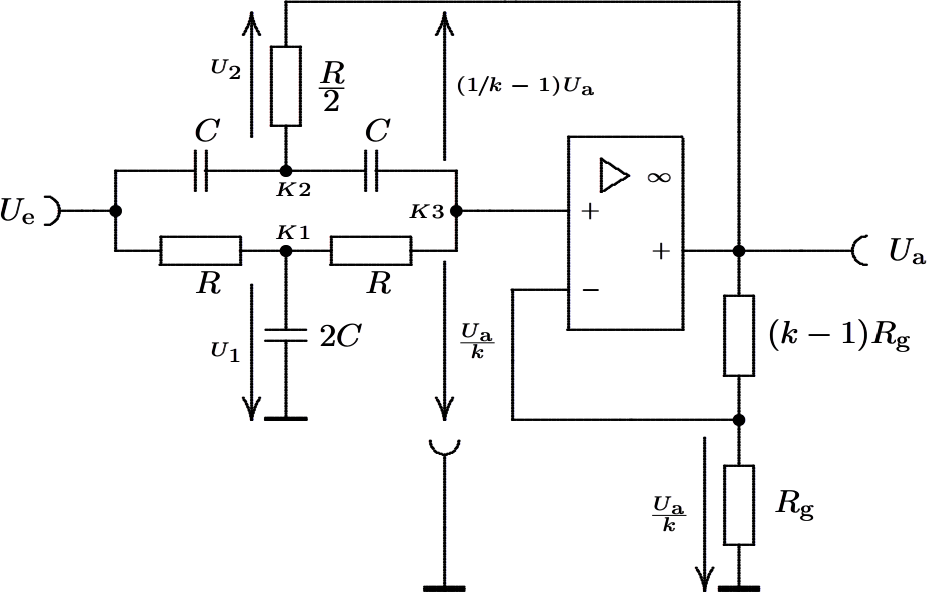
\includegraphics[width=\textwidth]{bandsperre.png}
\caption{Bandsperre mit OPV} \label{img:band}
\end{figure}
\subsection{Dimensionierung}
Für die gezeigte Bandsperre war eine Resonanzfrequenz von $f\ix{r}\approx\unit[10]{kHz}$ gefordert. Zusätzlich zu dieser, welche den nicht-invertierenden Eingang ansteuert, kommt ein invertierender Verstärker zum Einsatz. Die gesuchten Gegenkopplungsfaktoren ergeben sich aus dem Verhältnis der Spannungsteilerwiederstände $R\ix{g}$ und $ \left(k-1\right)R\ix{g}$. Damit folgt:
\begin{align*}
U_-=\frac{\left(k-1\right)R\ix{g}}{\left(k-1\right)R\ix{g}+R\ix{g}}\cdot U\ix{a}=\left(1-\frac{1}{k}\right)\cdot U\ix{a}
\end{align*}
Für die Kopplungsfaktoren $k=1$ bzw. $k=2$ verschwindet oder halbiert sich die rückgekoppelte Ausgangsspannung gerade. Aus der Definition der Resonanzfrequenz $f\ix{r}=\left(2\pi R C\right)^{-1}$ und der Forderung, dass der Ausgang nicht zu hochohmig belastet werden kann, folgt die Wahl von $R$, $C$ und $R\ix{g}$.
\section{Durchführung}
\subsection{Messgeräte}
Für die Messungen an der Bandsperre wurde ausschließlich das Oszilloskop \textsc{Hameg HM1508-2} verwendet. Die Speisespannung lieferte das Strom-/Spannungsversorgungsgerät \textsc{Tektronix PS 280} und die Eingangssignale wurden mit dem Funktionsgenerator \textsc{Tektronix AFG 3022B} erzeugt.
\subsection{Oszillogramme}
Messaufgabe 11 forderte die Aufnahme von Oszillogrammen von Ein- und Ausgangsspannungen bei rechteckförmigen Eingangssignalen mit Grundfrequenzen $f\lessapprox f\ix{r}$, $f\gtrapprox f\ix{r}$, $f\lessapprox \frac{f\ix{r}}{3}$ und $f\gtrapprox \frac{f\ix{r}}{3}$. Dabei war die Gegenkopplung $k\approx2$.
\begin{figure}[H]
\centering
\begin{subfigure}[b]{.41\textwidth}
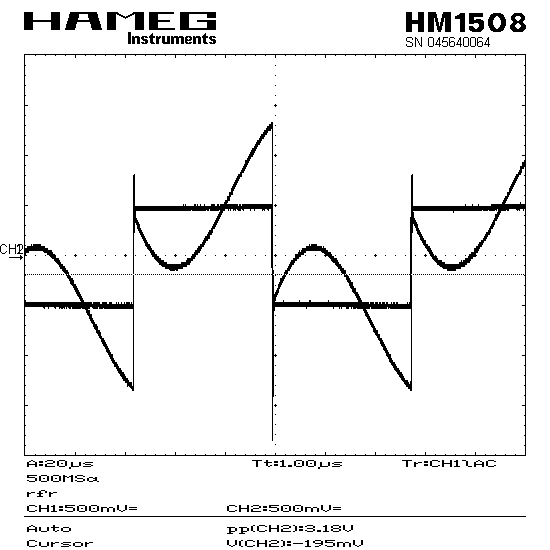
\includegraphics[width=\textwidth]{SCR00010.png}
\subcaption{$f\approx \unit[9]{kHz}\lessapprox f\ix{r}$}
\end{subfigure}
\begin{subfigure}[b]{.41\textwidth}
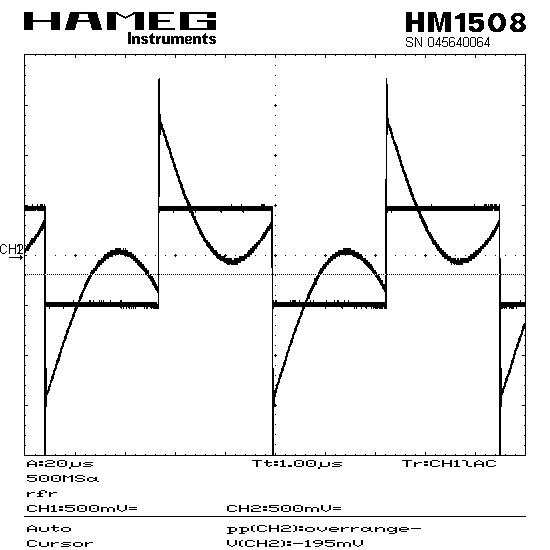
\includegraphics[width=\textwidth]{SCR00011.png}
\subcaption{$f\approx \unit[11]{kHz}\gtrapprox f\ix{r}$}
\end{subfigure}
\begin{subfigure}[b]{.41\textwidth}
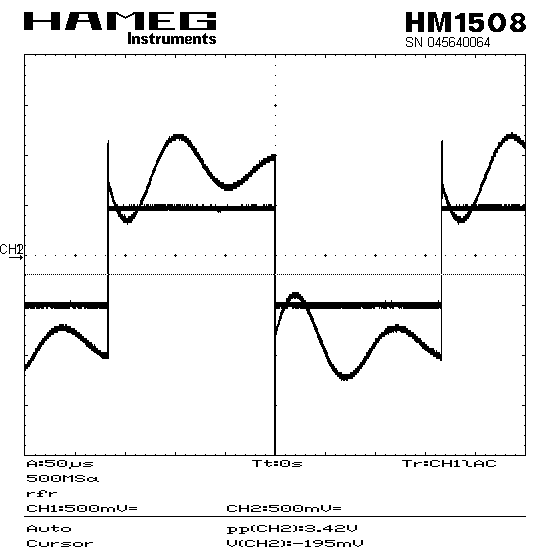
\includegraphics[width=\textwidth]{SCR00013.png}
\subcaption{$f\approx \unit[3]{kHz}\lessapprox \frac{f\ix{r}}{3}$}
\end{subfigure}
\begin{subfigure}[b]{.41\textwidth}
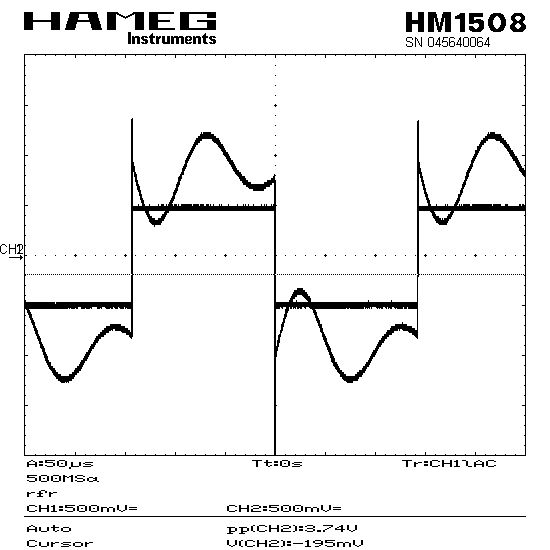
\includegraphics[width=\textwidth]{SCR00012.png}
\subcaption{$f\approx \unit[3,5]{kHz}\gtrapprox \frac{f\ix{r}}{3}$}
\end{subfigure}
\caption{Oszillogramme zur Messaufgabe 11, Eingang: rechteckförmiges Signal}
\end{figure}
\subsection{Messwerte}
Weiterhin wurden die Frequenzgänge der Phasenverschiebung und der Übertragungsfunktion bei Gegenkopplungen $k=1$ und $k\approx2$ aufgenommen.
\begin{figure}[H]
\centering
\begin{subfigure}[b]{\textwidth}
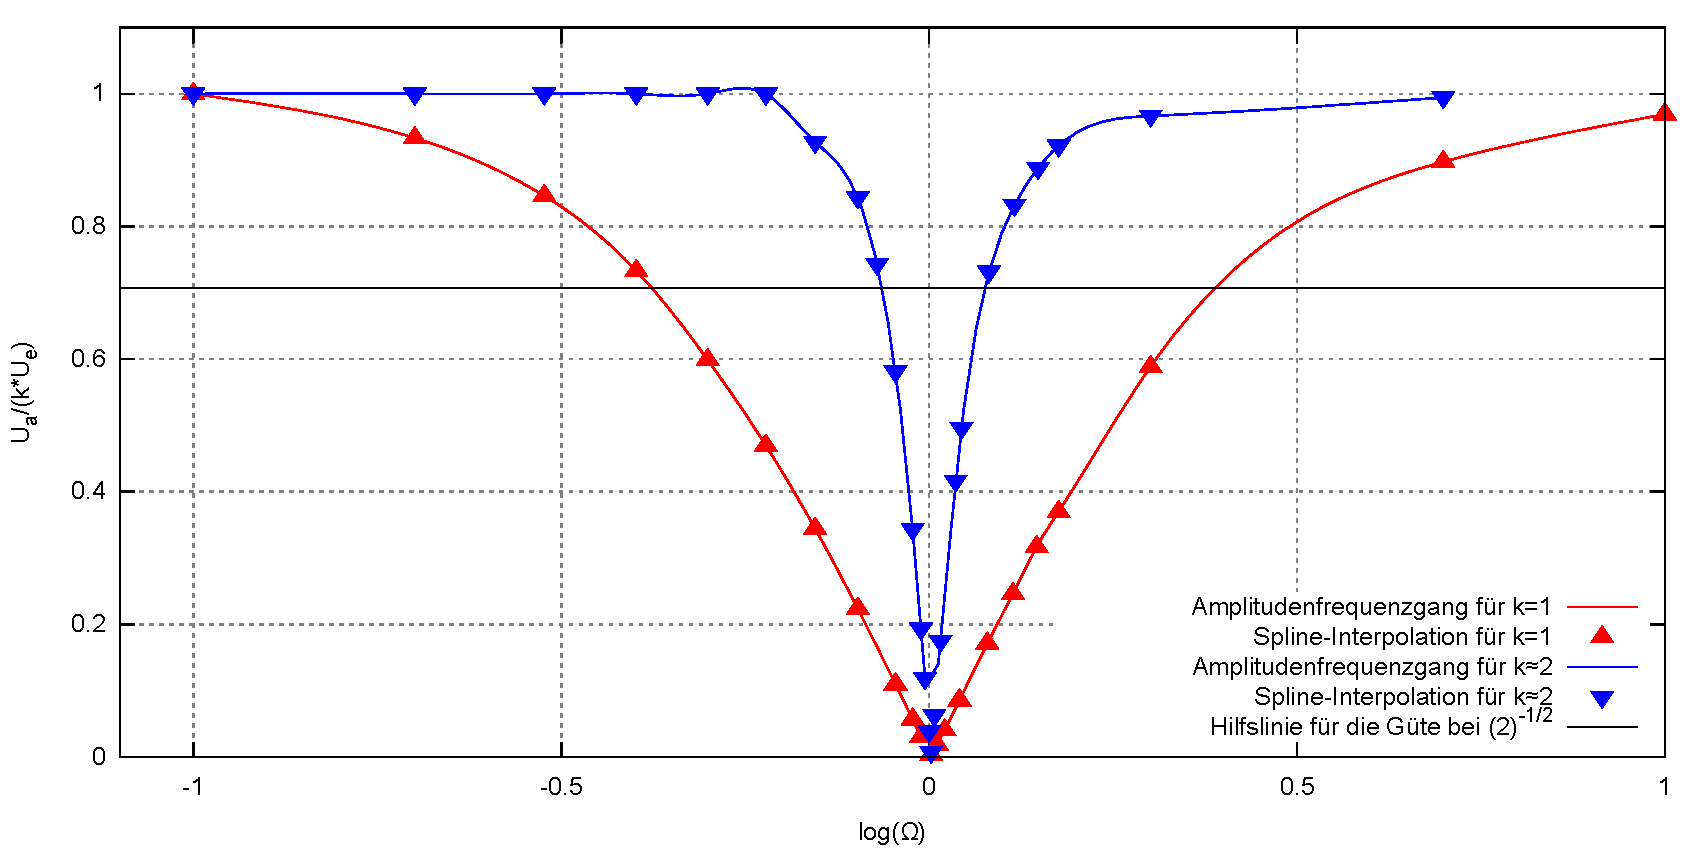
\includegraphics[width=\textwidth]{sfg.pdf}
\subcaption{Amplitudenfrequenzgänge}
\end{subfigure}
\begin{subfigure}[b]{\textwidth}
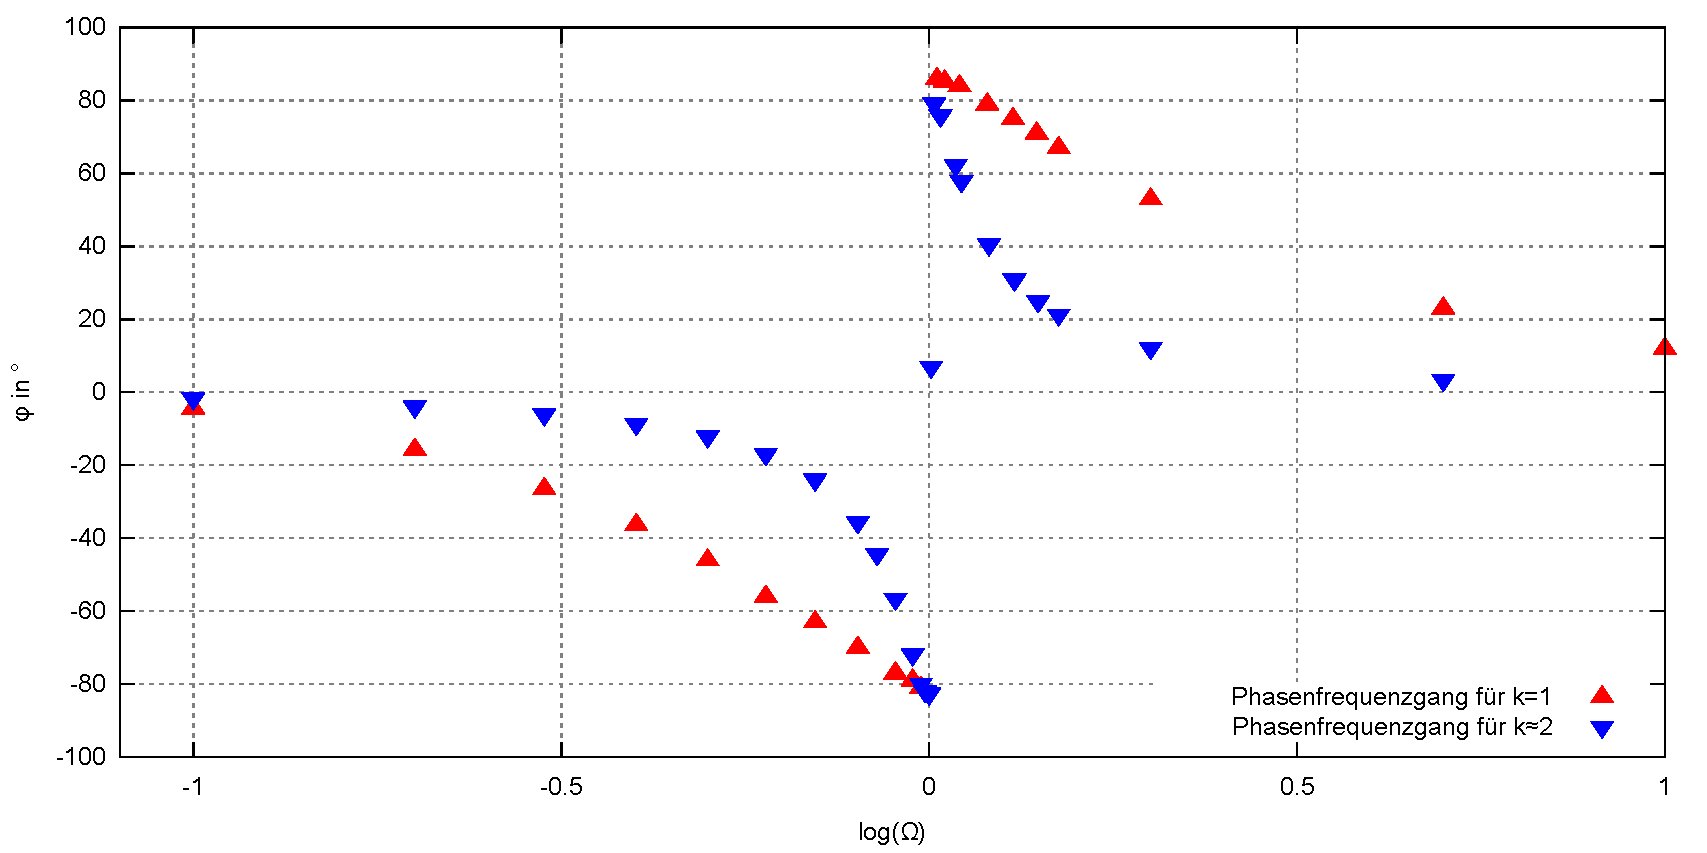
\includegraphics[width=\textwidth]{pfg.pdf}
\subcaption{Phasenfrequenzgänge}
\end{subfigure}
\caption{Diagramme der Messwerte}
\end{figure}
\section{Auswertung}

\section{Anhang}
Die originalen Messwert-Aufzeichnungen liegen bei.
\end{document}